\chapter{Opis projektnog zadatka}
		
		
		\indent Cilj ovog projekta je razviti programsku podršku za stvaranje web aplikacije "Maketa shop" koja se sastoji od dva glavna dijela. 
		\indent Prvi dio omogućuje objavljivanje sadržaja vezanih uz izradu maketa. Sadržaj je u obliku priča koje se sastoje od slika, videa, teksta ili kombinacija svega navedenog koji prate proces izrade maketa. Same priče objavljuje administrator dok registrirani korisnici iste mogu predlagati. Postoji mogućnost dodavanja komentara na priče, koje mogu ostavljati registrirani i neregistrirani korisnici. \\
		\indent Drugi dio je \textit{webshop} na kojemu korisnici mogu naručivati makete. Sam \textit{shop} je standardna web-trgovina sa svim funkcionalnostima koje korisnik očekuje od takve stranica. Razlika između "Maketa shopa" i drugih web-trgovina je u mogućnosti naručivanja maketa po vlastitim zamislima. Korisnik može maketaru (administratoru) poslati nacrte i opise makete kakvu želi, a maketar taj zahtjev može prihvatiti ili odbiti. Kada se obje strane slože oko cijene, proces se nastavlja na standardan način.
		
		\begin{figure}[H]
			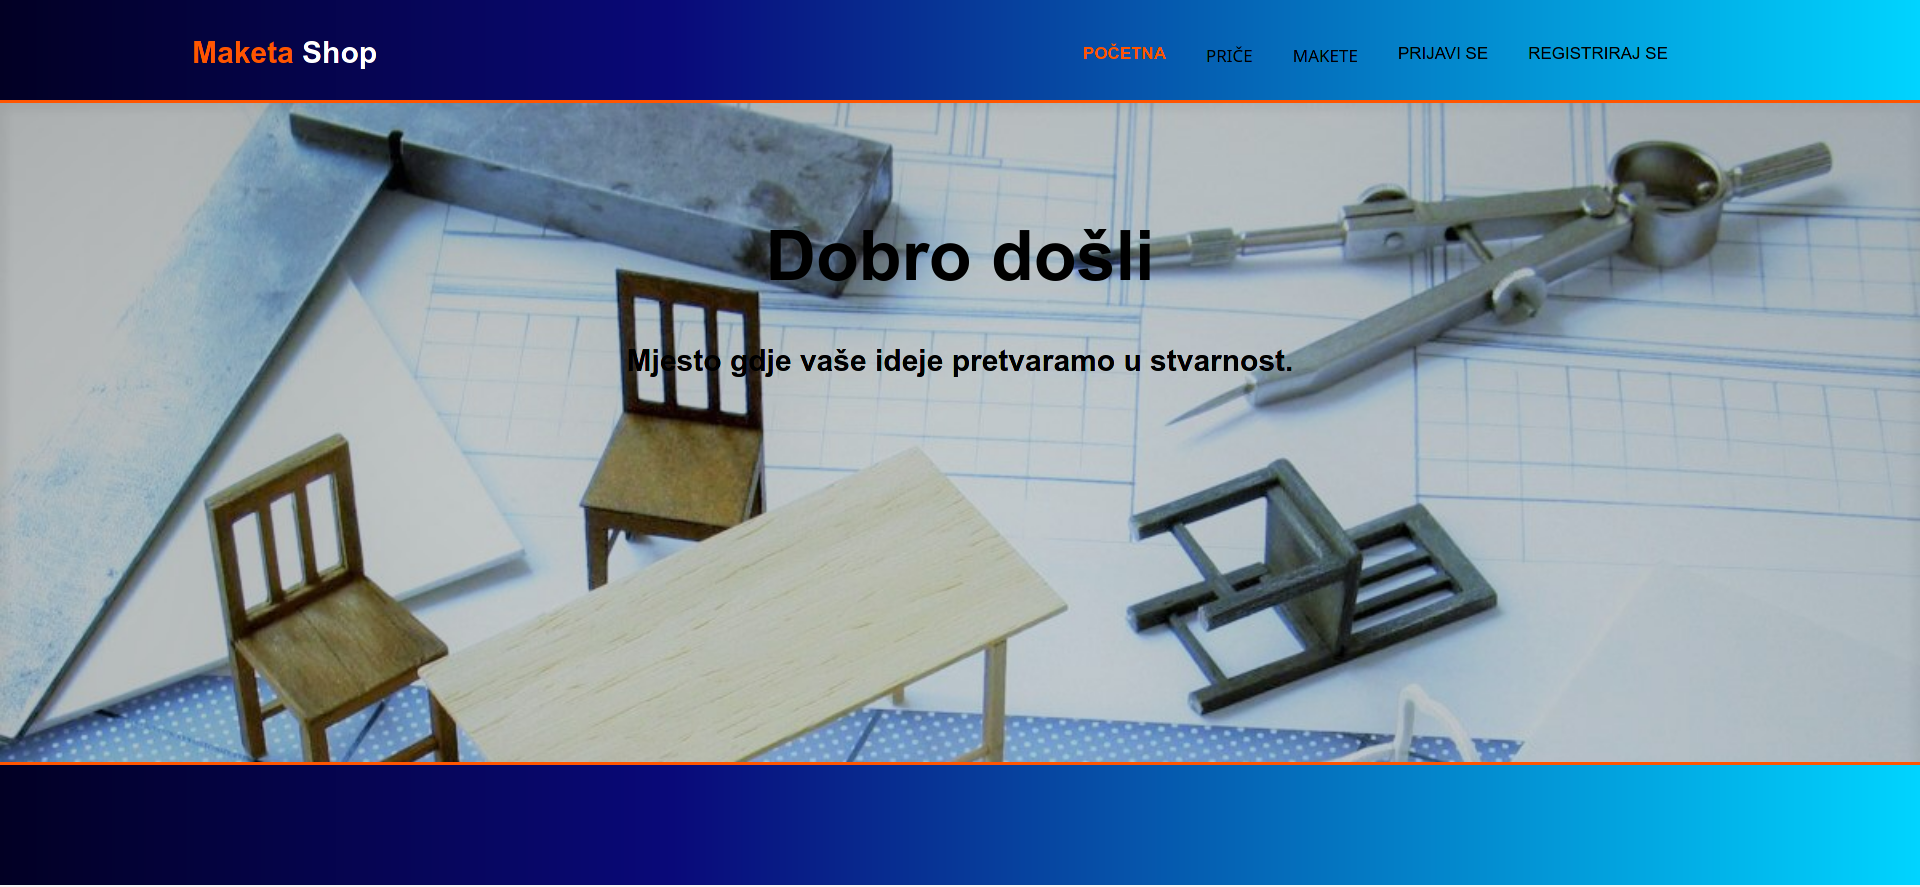
\includegraphics[width=.9\linewidth]{slike/20201112_182209.png}
			\centering
			\caption{Početna stranica}
			\label{fig:opis1}
		\end{figure}
	
		Aplikaciji mogu pristupiti registrirani i neregistrirani korisnici. Pri prvom ulasku u aplikaciju, svaki korisnik ima opciju Registracije, te prijavljivanja s postojećim računom. Aplikacija registriranim korisnicima pruža mogućnost spremanja informacija kako se ne bi trebali svaki put prijavljivati i unositi osobne podatke prilikom plaćanja narudžbe. Podaci potrebni za kreiranje korisničkog računa su:
		
		\begin{itemize}
			\item korisničko ime (mora biti jedinstveno)
			\item e-mail adresa (mora biti jedinstvena)
			\item lozinka
		\end{itemize} 	
	
		\begin{figure}[H]
			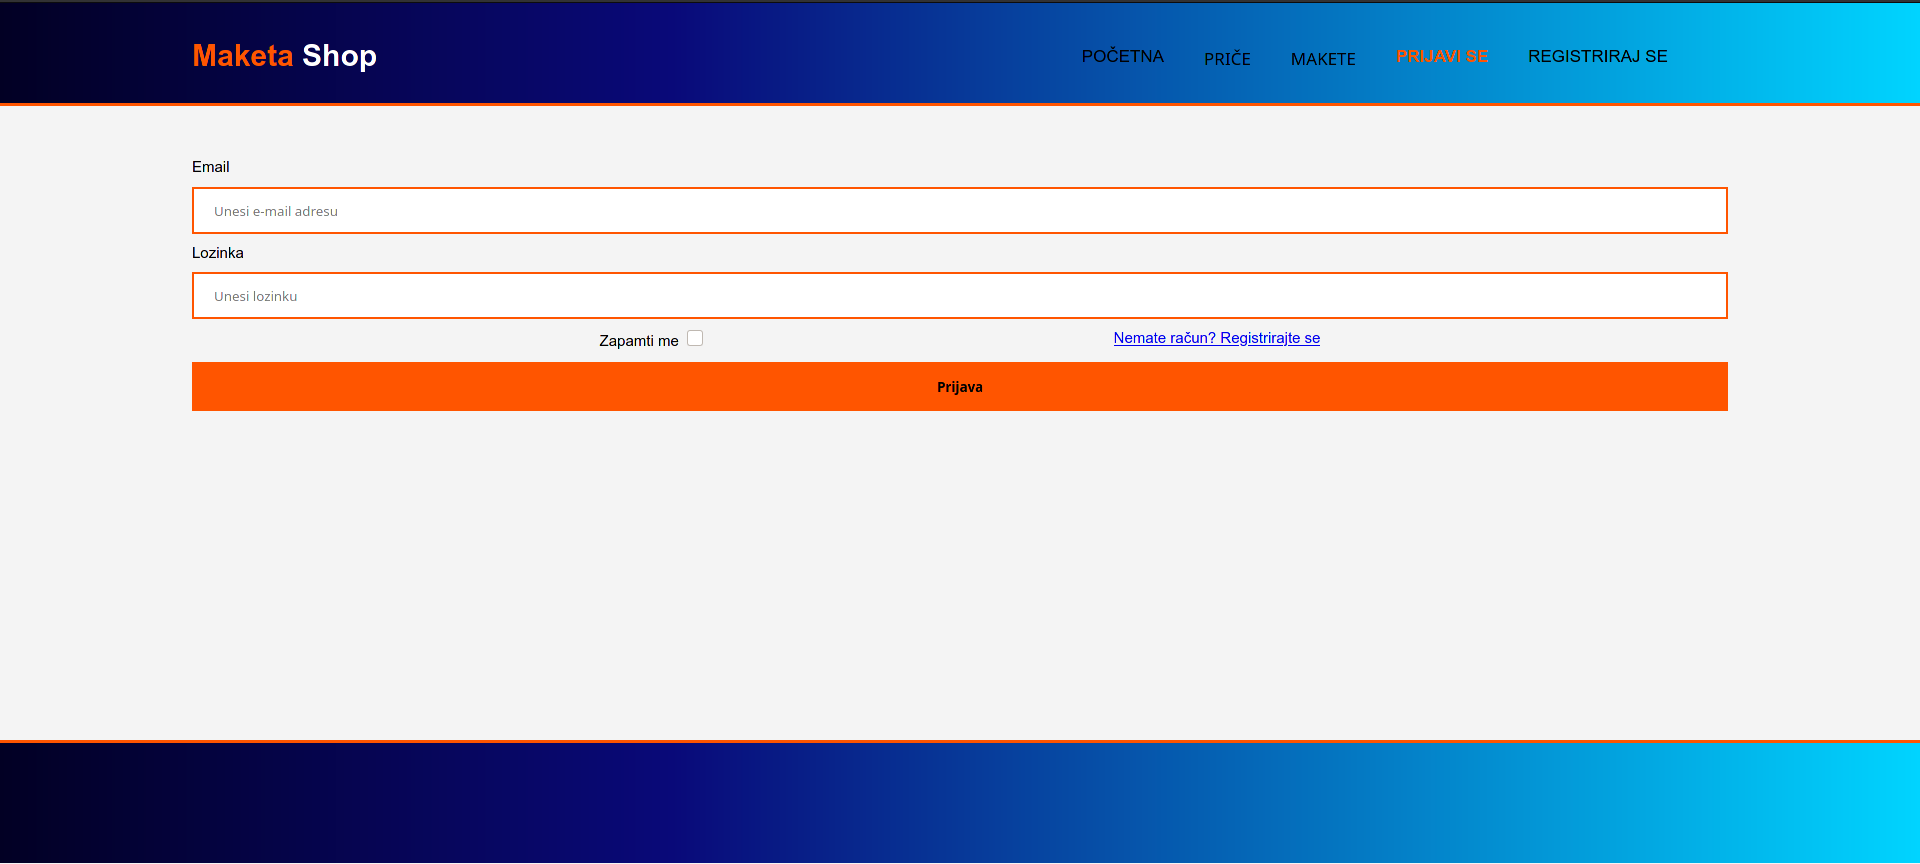
\includegraphics[width=.9\linewidth]{slike/20201112_182228.png}
			\centering
			\caption{Prijava u sustav}
			\label{fig:opis2}
		\end{figure}
	
		\begin{figure}[H]
			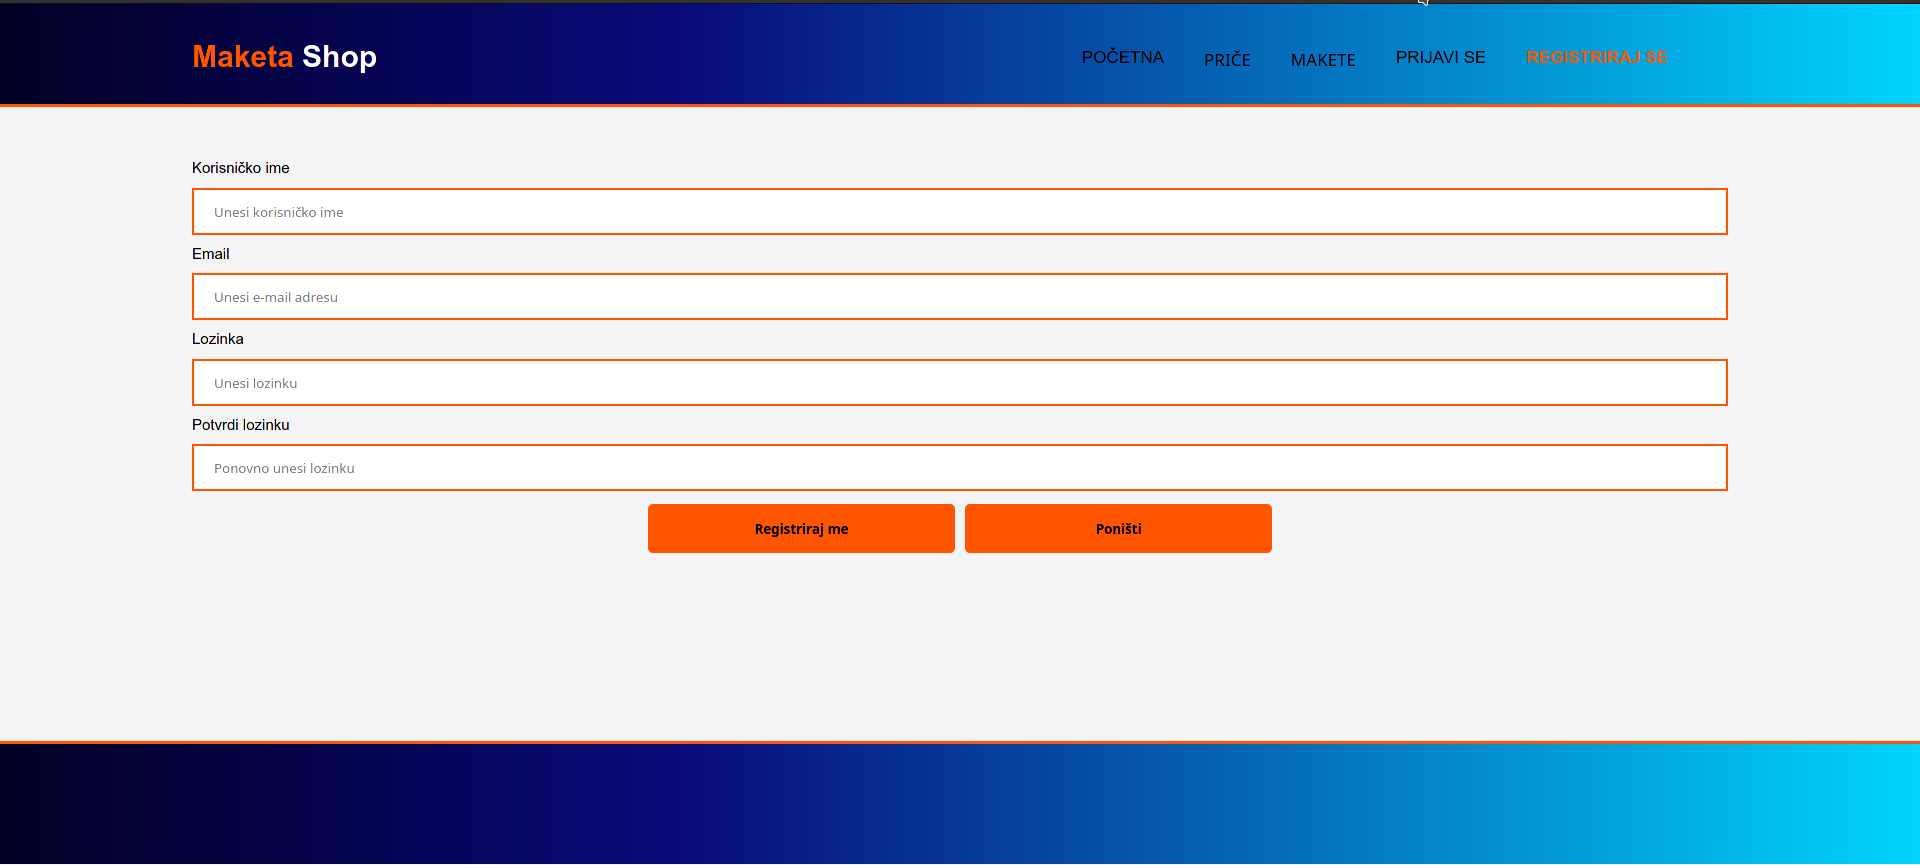
\includegraphics[width=.9\linewidth]{slike/20201112_182312.png}
			\centering
			\caption{Registracija}
			\label{fig:opis3}
		\end{figure}
	
		Korisničko ime je javno svima dok za druge podatke korisnik određuje hoće li biti privatni ili javni.\\
		
		Aplikacija pruža opciju kupnju standardne makete. Svaka maketa je detaljno opisana (dimenzija, materijal, boja) te se korisniku pruža mogućnost odabira nekoliko različitih materijala koji bi se koristili u izradi makete. Cijene će se razlikovati ovisno o biranim materijalima, te su one unaprijed određene od strane administratora. Također korisniku je omogućeno naručivanje makete prema vlastitim skicama. Atributi makete će se unositi u formular gdje se definira opis makete, dimenzija i materijal za izradu. Nakon što se formular ispuni administratoru se šalje obavijest, te ona ima mogućnost pregleda zahtjeva te određuje cijenu za tu maketu, koju korisnik može prihvatiti ili odbiti. \\
		Plaćanje se 'odvija' pomoću formulara čijim se ispunjavanjem simulira online plaćanje. Podaci uneseni u formular se trebaju spremati, te se registriranim korisnicima nakon prvog plaćanja formular automatski puni. Povijest svih transakcija se treba spremati i pamtiti te mora biti dostupna administratoru. \\
		
		Postoje 3 vrste korisnika u aplikaciji:
		\begin{itemize}
			\item \underline{Neregistrirani korisnik} je osnovna uloga u web aplikaciji. Neregistrirani korisnik ima mogućnost kupovine maketa, međutim njegovi podaci se neće automatski popunjavati prilikom svake sljedeće kupovine, omogućeno mu je komentiranje na postojeće priče međutim nema mogućnosti predlaganja novih priča.
			\item \underline{Registrirani korisnik} je uloga koja se ostvaruje prilikom registracije i prijave. Registrirani korisnik ima sve mogućnosti kao i neregistrirani korisnik međutim za njega postoji mogućnost automatskog ispunjavanja podataka prilikom plaćanja, te mogućnost predlaganja priča administratoru, također ima mogućnost naručivanja maketa prema vlastitim specifikacijama.
			\item \underline{Administrator} je uloga koja se dodjeljuje jednoj osobi te on ima najveće ovlasti. Administrator je jedina osoba koja može objavljivati priče, samostalno ili na prijedlog registriranih korisnika. Također ima mogućnost pregleda proteklih transakcija. Administratoru je omogućena zabrana pristupa registriranim korisnicima.
		\end{itemize}